\section{Art Style}
The art style of \ourgame{} is largely influenced by the individual styles and previous works of \ourteam{}'s art department.

\begin{figure}[H]
\centering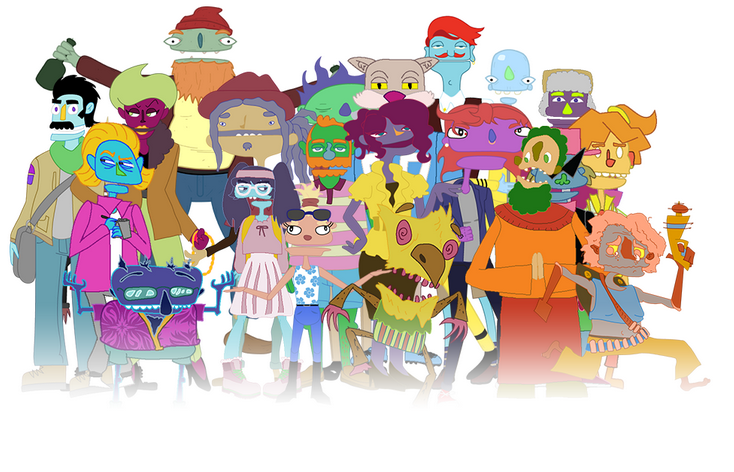
\includegraphics[width=0.7\linewidth]{images/art_style}
\end{figure}

\clearpage
Ian's characters, shown in Figure~\ref{fig:i1}, were a starting point from which \ourgame{}'s character designs stemmed from. \ourgame{}'s character's concepts were also inspired by Michael's art for a previous game, \textit{This Is Our Game And I'm Out Of Ideas}, seen in Figure~\ref{fig:m1}, where characters were broken into components and moved strangely, possessing inhuman freedom in joint movement. The design of the characters were also influenced by \textit{Stick it to the Man}, seen in Figure~\ref{fig:artref1}, with jaws that are separate from their upper jaw.

\begin{figure}[H]
\centering %
\begin{subfigure}{.3\textwidth}
\centering
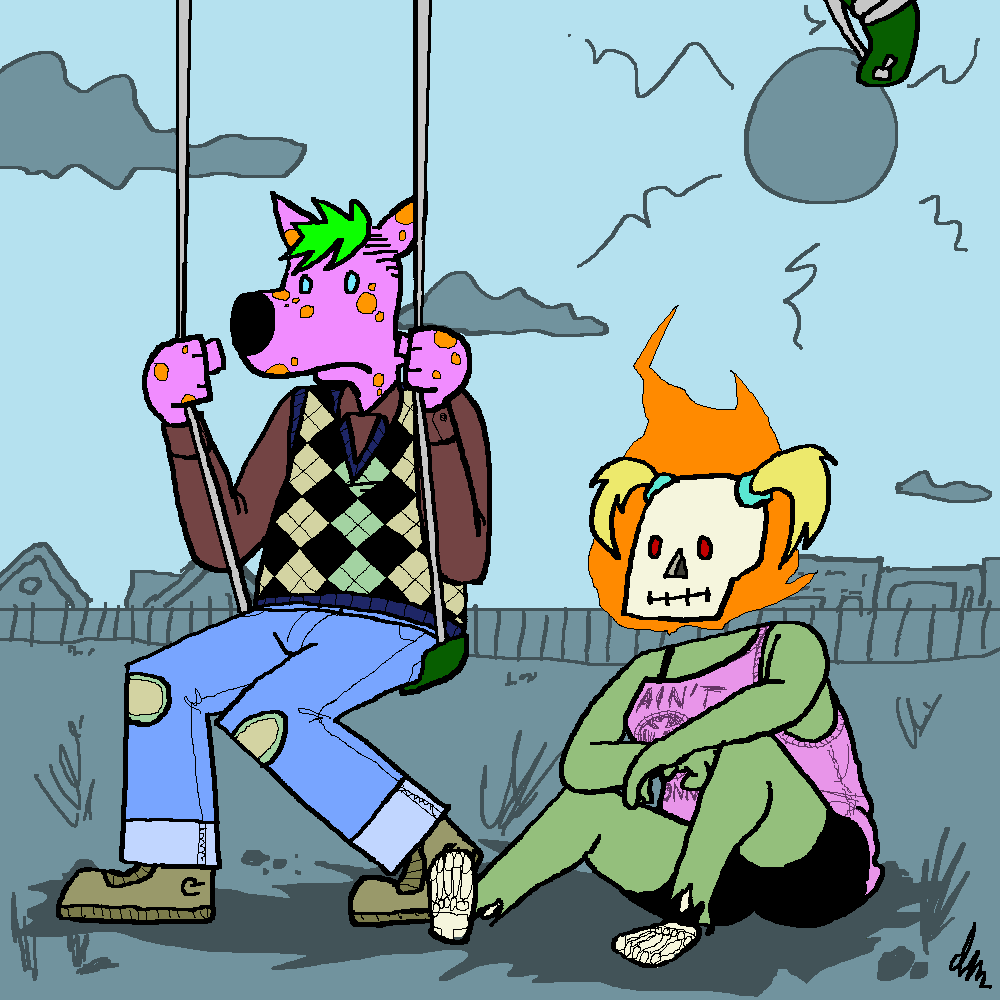
\includegraphics[width=.9\linewidth]{images/ref_IAN01}
 	\caption{Comic - \textit{Monster Friends in "Halloween"}}
\label{fig:i1}
\end{subfigure} %
\begin{subfigure}{.59\textwidth}
\centering
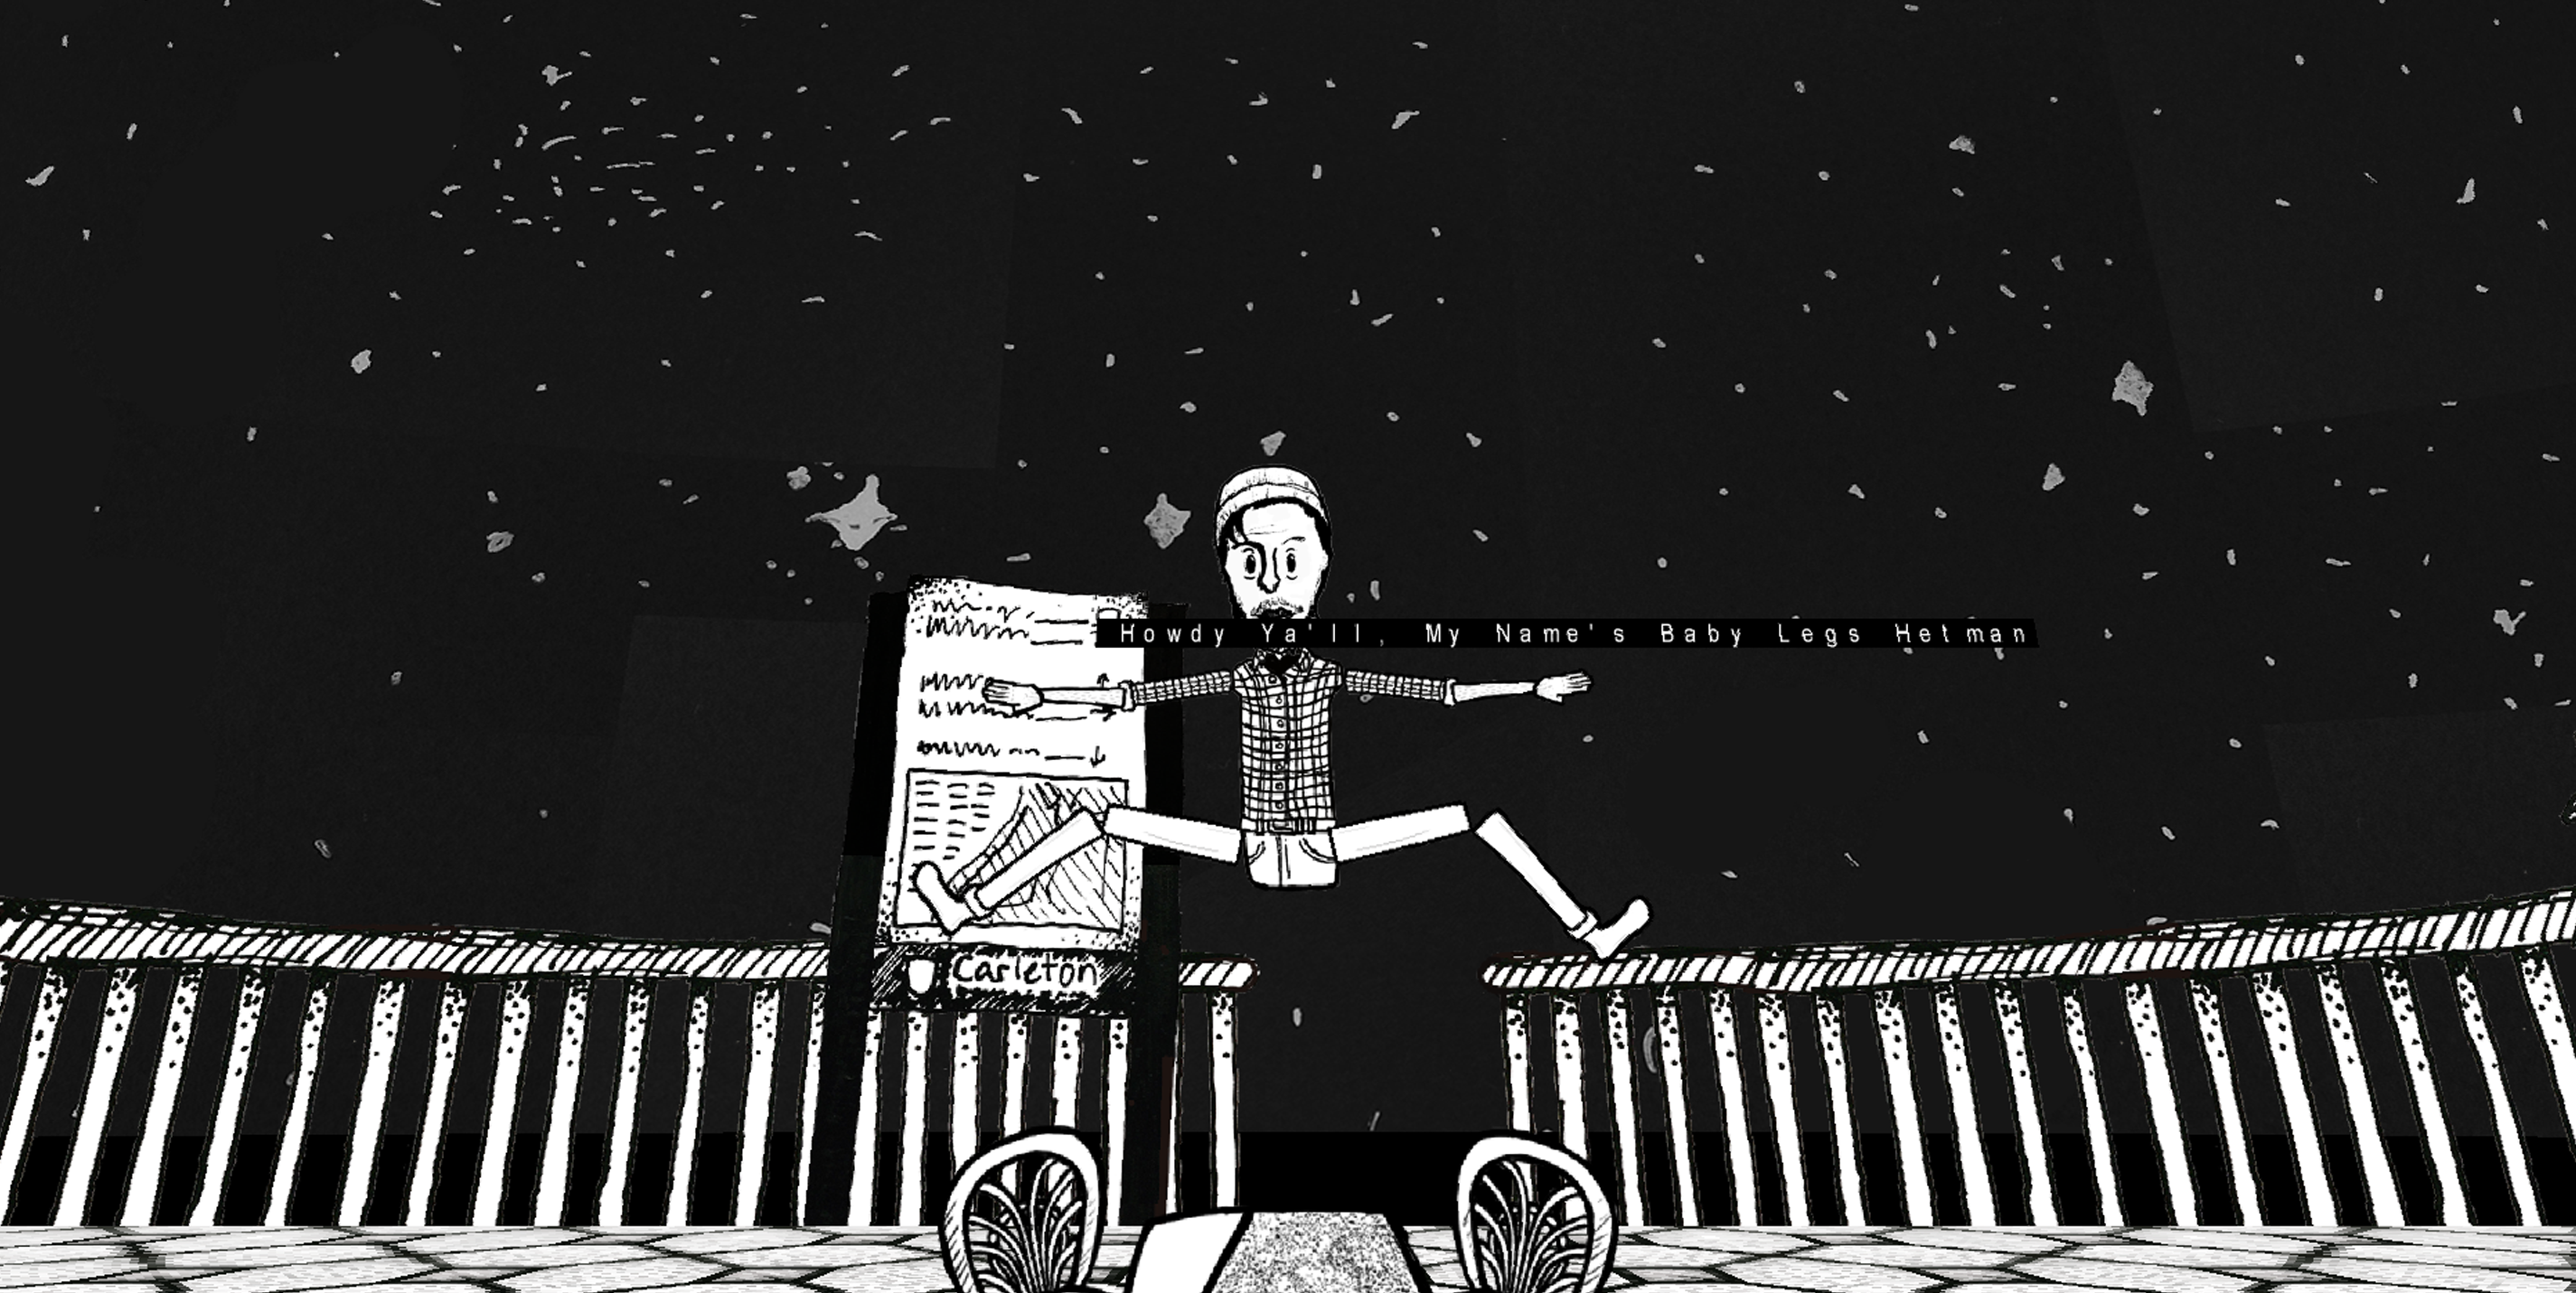
\includegraphics[width=.9\linewidth]{images/ref_MICHAEL03}
\caption{Character in TIOGAIOOI}
\label{fig:m1}
\end{subfigure} %
\begin{subfigure}{.45\textwidth}
  \centering
  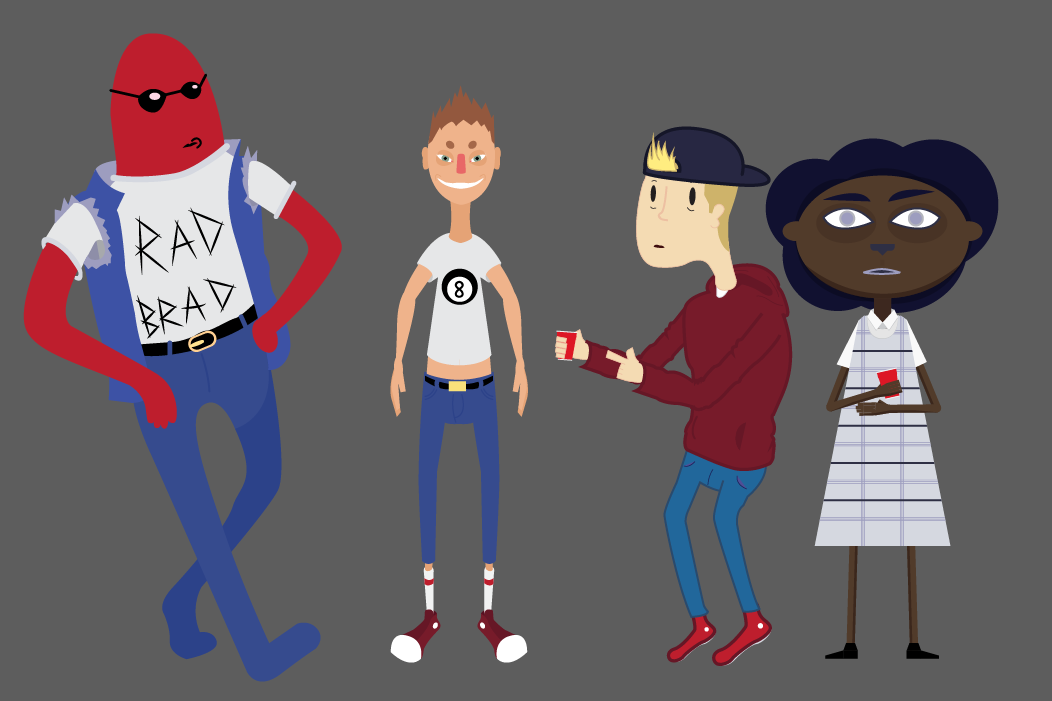
\includegraphics[width=.9\linewidth]{images/ref_MICHAEL04}
  \caption{Initial Character Ideas}
  \label{fig:m4}
\end{subfigure}
\label{fig:mstyle}
\end{figure}

The base structure for the characters can be described as bipedal humanoids. While many of the characters are humans, there are also a variety of mythological creatures and mechanical beings included. Anthropomorphic and folklore themes were explored and incorporated into some of the character designs, presented as mundane beings sporting modern clothing. The mixture of human and non-human characters creates a more surreal style, similar to that of \textit{Psychonauts} in Figure~\ref{fig:artref2}.

Tall characters tend to be more lanky and creepy, with irregular human body proportions emphasizing long and thin limbs. These can be seen in \ourgame{}'s early concept art in Figure~\ref{fig:m4}. Similarly, short characters have more blocked out and stubby limbs. This gives them a more grounded appearance. Some of the human characters sport distinctive clothing based off modern subcultures to exaggerate their personalities. Details in apparel and fashion statements gives the characters more distinctive features.

The overall style of \ourgame{} mixes 2D and 3D elements, an approach taken by other similar games such as \textit{Burrito Galaxy} and \textit{Little Party}, shown in Figure\ref{fig:artref3} and Figure~\ref{fig:artref4}. The scrolling speech bubbles, one of the highlights of \ourgame{}'s UI, was inspired by \textit{Night in the Woods: Lost Constellation}, seen in Figure~\ref{fig:artref5}.

\begin{figure}[H]
\centering %
\begin{subfigure}{.4\textwidth}
\centering
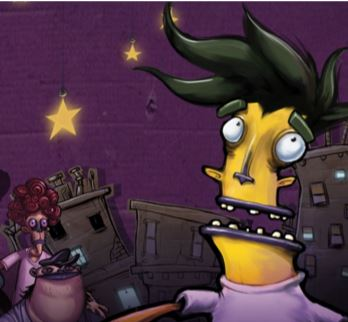
\includegraphics[width=.9\linewidth]{images/ref_sittm}
\caption{\textit{Stick it to the Man}}
\label{fig:artref1}
\end{subfigure} %
\begin{subfigure}{.4\textwidth}
\centering
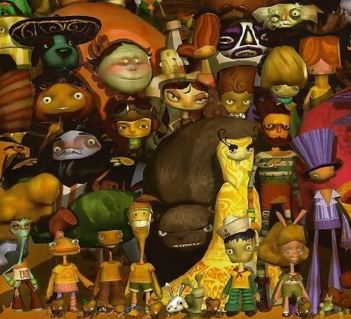
\includegraphics[width=.9\linewidth]{images/ref_psychonauts}
\caption{\textit{Psychonauts}}
\label{fig:artref2}
\end{subfigure} %
\begin{subfigure}{.33\textwidth}
\centering
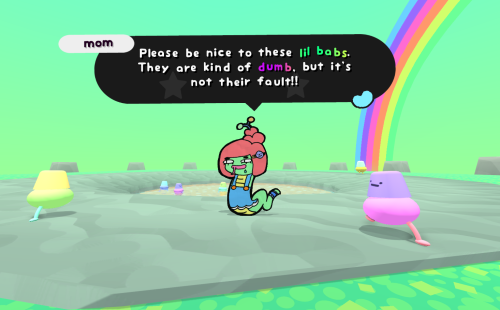
\includegraphics[width=.9\linewidth]{images/ref_burgal}
\caption{\textit{Burrito Galaxy}}
\label{fig:artref3}
\end{subfigure} %
\begin{subfigure}{.33\textwidth}
\centering
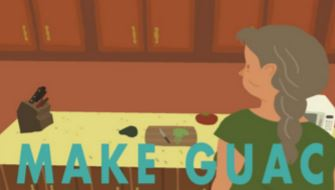
\includegraphics[width=.9\linewidth]{images/ref_litpar}
\caption{\textit{Little Party}}
\label{fig:artref4}
\end{subfigure} %
\begin{subfigure}{.33\textwidth}
\centering
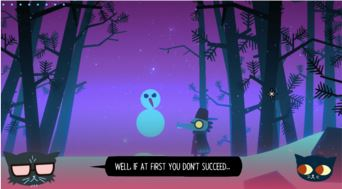
\includegraphics[width=.9\linewidth]{images/ref_nitw}
\caption{\textit{Night in the Woods: Lost Constellation}}
\label{fig:artref5}
\end{subfigure}
\end{figure}